% Generated by scripts/make_explanation_figures.py from experiment_0013 (do not edit by hand).
% Model: COVER
\documentclass[tikz,border=3pt]{standalone}
\usepackage[T1]{fontenc}
\usepackage[utf8]{inputenc}
\usepackage{newtxtext,newtxmath}
\usetikzlibrary{positioning,arrows.meta,calc}

\definecolor{neural}{HTML}{2F6DB5}
\definecolor{neuralbg}{HTML}{E8F0FA}
\definecolor{logic}{HTML}{2E8B57}
\definecolor{logicbg}{HTML}{E6F4EC}
\definecolor{relneg}{HTML}{C0392B}

\tikzset{
  tok/.style={draw=neural!80, fill=white, rounded corners=1.5pt, inner sep=1.6pt, font=\scriptsize,
              minimum height=4mm, anchor=base},
  htok/.style={tok, fill=neural!12},
  stok/.style={tok, draw=black!25, text=black!45},
  aedge/.style={line width=#1, draw=logic},
  cedge/.style={line width=#1, draw=relneg},
  ledge/.style={line width=#1, draw=neural, densely dashed},
  rlab/.style={font=\tiny, fill=white, inner sep=0.6pt},
}
\newcommand{\bars}[4]{%
  \fill[logic]  (#1-0.17,0.05) rectangle ++(0.15,{0.8*#2});
  \fill[relneg] (#1+0.02,0.05) rectangle ++(0.15,{0.8*#3});
  \node[font=\tiny, anchor=north] at (#1-0.095,0.03) {$s$};
  \node[font=\tiny, anchor=north] at (#1+0.095,0.03) {$c$};
  \node[font=\tiny, anchor=north] at (#1,-0.22) {$#2\,/\,#3$};
  \node[font=\tiny, anchor=north, text=black!60] at (#1,-0.47) {$\omega{=}#4$};
}
\newcommand{\sbar}[3]{%
  \fill[logic]  (#1-0.075,0.05) rectangle ++(0.15,{0.8*#2});
  \node[font=\tiny, anchor=north] at (#1,0.03) {$s$};
  \node[font=\tiny, anchor=north] at (#1,-0.22) {$#2$};
  \node[font=\tiny, anchor=north, text=black!60] at (#1,-0.47) {$\omega{=}#3$};
}
\providecommand{\Pcov}{P_{\mathrm{cov}}}
\providecommand{\Pnc}{P_{\neg\mathrm{conf}}}
\providecommand{\E}{\textsc{e}}
\providecommand{\N}{\textsc{n}}
\providecommand{\C}{\textsc{c}}

\begin{document}
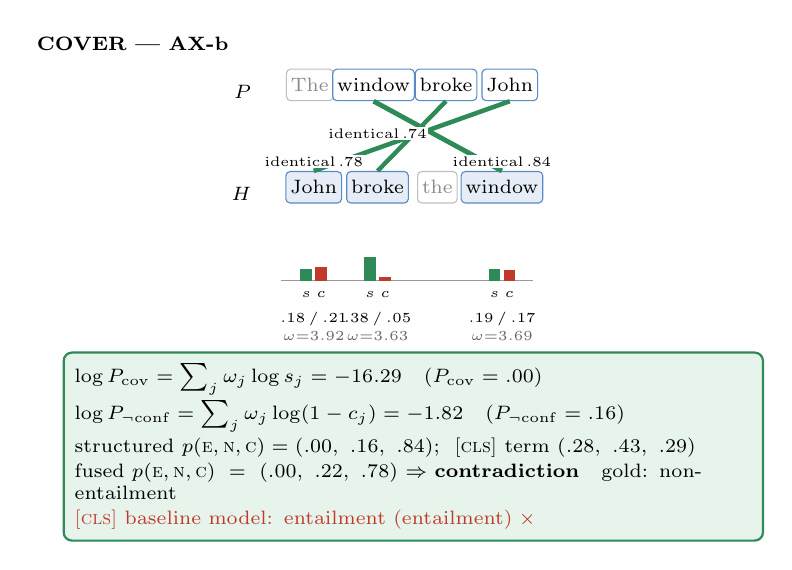
\begin{tikzpicture}
\begin{scope}[xshift=2.57cm]
\node[font=\scriptsize\itshape, anchor=east] at (-0.35,2.45) {$P$};
\node[font=\scriptsize\itshape, anchor=east] at (-0.35,1.15) {$H$};
\node[stok] (pw0) at (0.27,2.45) {The};
\node[tok] (p2) at (1.08,2.45) {window};
\node[tok] (p3) at (2.00,2.45) {broke};
\node[tok] (p4) at (2.81,2.45) {John};
\node[htok] (h8) at (0.32,1.15) {John};
\node[htok] (h9) at (1.13,1.15) {broke};
\node[stok] (hw2) at (1.89,1.15) {the};
\node[htok] (h11) at (2.71,1.15) {window};
\draw[aedge=1.64pt] (h8.north) -- (p4.south);
\draw[aedge=1.59pt] (h9.north) -- (p3.south);
\draw[aedge=1.75pt] (h11.north) -- (p2.south);
\node[rlab, anchor=south] at (0.32,1.47) {identical\,.78};
\node[rlab, anchor=south] at (1.13,1.83) {identical\,.74};
\node[rlab, anchor=south] at (2.71,1.47) {identical\,.84};
\draw[black!40] (-0.1,0.05) -- (3.11,0.05);
\bars{0.32}{.18}{.21}{3.92}
\bars{1.13}{.38}{.05}{3.63}
\bars{2.71}{.19}{.17}{3.69}
\end{scope}
\node[draw=logic, fill=logicbg, rounded corners=3pt, line width=0.8pt, font=\scriptsize, align=left, anchor=north west, text width=8.60cm, inner sep=4pt] (agg) at (-0.3,-0.85) {%
  $\log\Pcov=\sum_j\omega_j\log s_j=-16.29$\quad($\Pcov=.00$)\\[1pt]$\log\Pnc=\sum_j\omega_j\log(1-c_j)=-1.82$\quad($\Pnc=.16$)\\[1pt]structured $p(\E,\N,\C)=(.00,\ .16,\ .84)$;\ \ \textsc{[cls]} term $(.28,\ .43,\ .29)$\\[1pt]fused $p(\E,\N,\C)=(.00,\ .22,\ .78)$ $\Rightarrow$ \textbf{contradiction}\quad gold: non-entailment\\[1pt]\textcolor{relneg}{\textsc{[cls]} baseline model: entailment (entailment) \texttimes}};
\node[font=\scriptsize\bfseries, anchor=south west] at (-0.75,2.85) {COVER --- AX-b};
\end{tikzpicture}
\end{document}
